
\documentclass{llncs}

\usepackage{float}
\usepackage{graphicx}
\usepackage{booktabs}
\usepackage{multirow}

% The title of the paper
\title{Capstone Proposal (Draft One): Offshore Wind Turbine Power Prediction and Wind Capacity Analysis Using LIDAR}

% The complete list of authors with their affiliations
\author{
Aditya Garapati\inst{1} \and
Charles Henderson\inst{1} \and
Carl Walenciak\inst{1}
Brian Waite\inst{1}
}

\institute{
Master of Science in Data Science, Southern Methodist University,
Dallas TX 75275 USA
\email{\{agarapati,chasehenderson,cwalenciak, bwaite\}@mail.smu.edu}
}

% Begin the document
\begin{document}

\maketitle              % typeset the title and author of the paper

% Reset the footnote counter
\setcounter{footnote}{0}
% The abstract environment uses the \begin{} and \end{} constructs to
% denote the beginning and ending of the abstract contents.
\begin{abstract}
Modeling techniques for the forecasting of wind speed using historical values observed by Light Detection and Ranging (LIDAR) sensors in an offshore context are described. Both univariate time series and multivariate time series modeling techniques leveraging meteorological data collected simultaneously with the LIDAR data are evaluated for potential contributions to predictive ability. Multiple time horizons are explored for optimal prediction accuracy and in accordance with identified use cases. Accurate and timely predictive ability of wind values are essential to the effective integration of wind power into existing power grid systems and allow for both the management of rapid ramp-up / ramp-down of base production capacity due to highly variable wind power production inputs and, over longer time horizons, integration of wind power into regional and national energy trading markets. Modeling successful indicates that <insert model type here> operating on data of a time interval of <insert minutes here> provide the most useful forecasts.

% Keywords may be used, but they are not required.
%\keywords{buoy LIDAR  \and wind turbine integration \and timeseries \and neural networks \and renewable energy.}
\end{abstract}


% Sections are denoted by the use of the \section{Section Name}
% command -- where "Section Name" is the name you give to the Section.
\section{Introduction}

At the end of 2019, the total installed wind power capacity in the United States was 105,583 Megawatts (MW) and the potential wind power capacity of the United States (at an 80 meter (m) turbine hub height) and its territories exceeded 10,640,000 MW. \cite{Energy2020} This makes wind the largest source of renewable energy in the country. \cite{AmericanWindEnergyAssociation2020} Successful integration of wind power resources into the national energy infrastructure, though, poses a number of challenges induced by the variability of wind energy availability including ramp events (rapid changes in demand or surplus of electrical production), induced wear and expanded emissions as a result of cycling traditional power production facilities up and down in their output, and increased management difficulty in balancing traditionally variable demand with a more stochastic input. \cite{osti_1097911} The ability to forecast wind values (speed and direction) is a key component of any solution to help energy operators successfully manage and integrate wind power into the existing energy grid.

\section{Proposal}

In this research, we seek to explore statistical time series, machine learning, and appropriate ensemble approaches to enable the forecasting of wind strength, and as a result theoretical power generation, at given wind turbine hub heights and rotor diameters with a forecasting horizon of 10 minutes up to 24 hours. These prediction windows are selected to allow models to support load balancing and reserve power management in the immediate near term (10 minutes to one hour) and "day-ahead" energy demand markets that support day-to-day grid planning. \cite{Ding2019}

\section{Wind Modeling}

In his book, "Data Science for Wind Energy", Prof. Ding identifies two primary approaches to wind forecasting. The first, Numerical Weather Prediction (NWP), is built on modeling of atmospheric data to produce outputs similar to the weather forecast used to predict daily weather and/or hurricane events. This model generally performs well on longer time scales, but requires intense computing power to execute. \cite{Ding2019} A second approach uses smaller scale, local sensor data to make statistical predictions based on single time series, sample-based modeling. \cite{Ding2019}

Our approach will be to first explore the techniques and modeling methods associated with the creation of time series based forecasting of wind at a specific site given historical wind values on specified intervals and with co-located sensor data of interest. If successful, we then hope to expand and improve our time series based forecast by incorporating features derived from data collected more traditionally in support of NWP modeling (such as regional temperature, wind speed, wind direction, barometric pressure, and similar values) and/or the development of ensemble machine learning approaches that can contribute to or compete with the time series prediction.

\subsection{Modeling Techniques}

\subsubsection{Univariate Modeling Techniques: Autoregressive Integrated Moving Average (ARIMA) Models}

Autoregressive Integrated Moving Average Models (ARIMA) models represent a univariate methodology to model timeseries data by identifying relationships between historical values occurring at specific "lags" (in the autoregressive or AR component) and by modeling forecast errors due to white noise components (moving average or MA component). ARIMA models rely on the underlying data meeting the conditions of stationarity to provide predictions and can incorporate components to "model out" non-stationary components by transforming the data with differencing and/or seasonal terms.

Using ARIMA modeling techniques to aid in forecasting wind values has been proven to be effective by Ding who describes techniques and requirements for preparing the data for ARIMA analysis. \cite{Ding2019}

\subsubsection{Multivariate Modeling Techniques: Long Short Term Memory (LSTM) Models}

LSTM models are a variant of Recurrent Neural Networks and offer the neural network to retain longer term memory and identify linkages to data that occur over longer time spans. This is ideal for timeseries analysis techniques where there may be correlation between inputs over long time scales that may be lost by other recurrent or deep neural networks as they learn. Further, LSTMs overcome the vanishing gradient problem whereby weight updates in Recurrent Neural Networks become insignificant. \cite{Pulver2016}

LSTMs overcome the problem of long term dependencies on the input vector by remembering information for a long period of time . LSTM uses series of gates to either remember the state or forget the state, training of the LSTM involves training the model on which state to remember and which state to forget.  An illustration of a LSTM cells is show below in Figure (need to ensure to update):

\begin{figure}
  \centering
  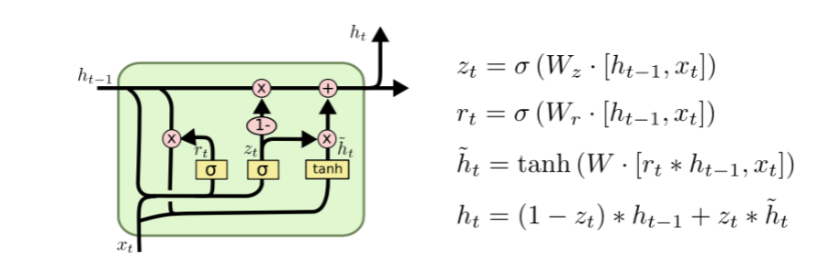
\includegraphics[width=0.75\textwidth]{LSTM_graphic.png}
  \caption{An example LSTM Node and Possible Activation Function}
  \label{fig:LSTMNode}
\end{figure}

LSTMs are capable of accepting multiple input variables and, as described above, we anticipate identifying contributions to wind speed modeling from associated meteorological data such as relative humidity, air pressure, surface wind speed, water temperature, as well as wind specific measurements such as vertical component wind speed and wind direction.

\section{Wind Buoy Program}

The U.S. Department of Energy (DOE) Office of Energy Efficiency and Renewable Energy (EERE) with the support of Pacific Northwest National Lab (PNNL) is currently supporting the deployment of an offshore wind energy evaluation effort using 20,000-pound buoys, known as WindSentinel, to measure meteorological and oceanographic parameters related to wind energy capacity. These buoys make use of Light Detection and Ranging (LIDAR) and other instruments to measure wind speed and direction, air and sea temperature, local barometric pressure, relative humidity, wave height and period, water conductivity, sub-surface currents, and other values in one second intervals. \cite{DOE}

Both historical and current buoy data from multiple locations are available to support model training and evaluation. Historical data includes data collected from between 2014 and 2017 in offshore locations near both Virginia and New Jersey. Active collection is ongoing off the coast of Massachusetts providing the opportunity to evaluate the model against real-world new data that is regularly being updated.

Additional data sources of interest include similarly collected 10-minute interval LIDAR data made available by the Danish firm Orsted from three unique offshore wind farm and meteorological station locations. \cite{Moore} Also, the Ding, 2019 text contains a number of data sets provided as exemplars of the methodologies described in the text from both on and off-shore locations that may be of additional interest, but which require exploration. \cite{Ding2019}

NWP weather data is available publicly from a number of sources including the U.S. National Weather Service. Availability of data of interest to our specific area of research is still being explored by the research team.

\section{Sensors}

\subsection{LIDAR Background} LIDAR technology is widely used as a mapping and survey technology from a wide variety of platforms (vehicles, aircraft, fixed point collection). The National Oceanic and Atmospheric Administration (NOAA), for example, has used the unique properties of infra-red and green laser LIDAR data to collect both topographic and bathymetric data remotely. \cite{noaa2012}

When used in the context of wind measurement, LIDAR is coupled with well understood Doppler shift calculations on the back-scatter reflections of aerosols -- small particulates contained in all air masses with diameters measured in fractions of microns -- to obtain wind speed and direction values at a number of different ranges near simultaneously. \cite{doppler_lidar} When deployed in an offshore wind measurement context, LIDAR has almost entirely replaced the deployment of traditional meteorological towers with traditional anemometer and wind-vane sensors that are generally fixed in the measurements they can provide based on their installation height and location. The ease of deployment too has resulted in significant cost savings and addressed safety concerns associated with offshore meteorological tower construction and operation. \cite{leosphere_2017}

\subsection{Vindicator and WindCube Sensors}

The first version of WindSentinel deployed during 2014-2017 used a Vindicator III LIDAR sensor to measure wind speeds at a variety of heights. The more recent ongoing survey in Massachusetts uses a WindCube sensor. Both sensors face challenges with noise induced by environmental concerns, the foremost being that the sensor is mounted on a gimble on a floating platform and is still subject to some pitch, roll, and yaw adjustments that impact the variance of its measurements.

Multiple approaches to address this are used by PNNL and DOE including a smoothing function applied to the 1 second interval data (1Hz data) or the chunking of data into 10 minute averages.

Work is ongoing within the group to explore the data, fields available, and the appropriate altitude that will allow the minimum amount of information lost and be most representative of the wind turbine use case. Further, we have completed functions to import data of both Vindicator III and WindCube output formats into our analytic environment.

\section{Exploratory Data Analysis} Wind speed is highly variable and driven by a number of both local and regional processes. As a first step to modeling over longer time horizons or larger datasets, the research team found it prudent to explore and fit a model for a single day as an initial step. In the below Figure, the plots show a single days time series realization, the associated autocorrelations and spectral density plots.

\subsection{ARIMA Modeling}
\begin{figure}
  \centering
  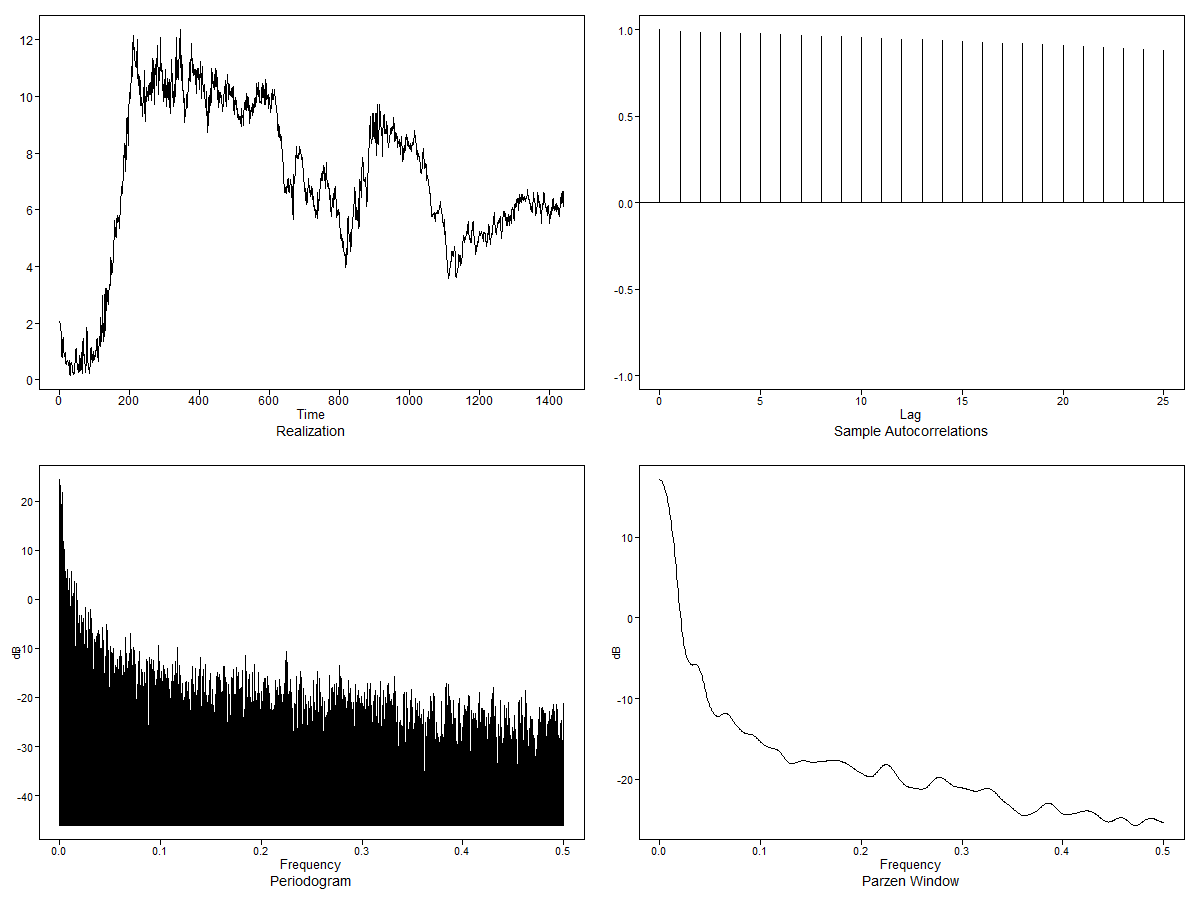
\includegraphics[width=0.75\textwidth]{apr_20_plot.png}
  \caption{Realization, Autocorrelation, Periodogram and Spectral Density Plot of Horizontal Wind Speed Values from 20 April 2016 at 1 Minute Intervals}
  \label{fig:Apr20Plot}
\end{figure}

As we can see, the plot demonstrates some significant wandering behavior in both the realization and the spectral density with a strong peak at f = 0. The extremely slow damping behavior observed in the ACF plot is an indication that the data is the result of a non-stationary process and should be differenced at least once before additional modeling.

\begin{figure}
  \centering
  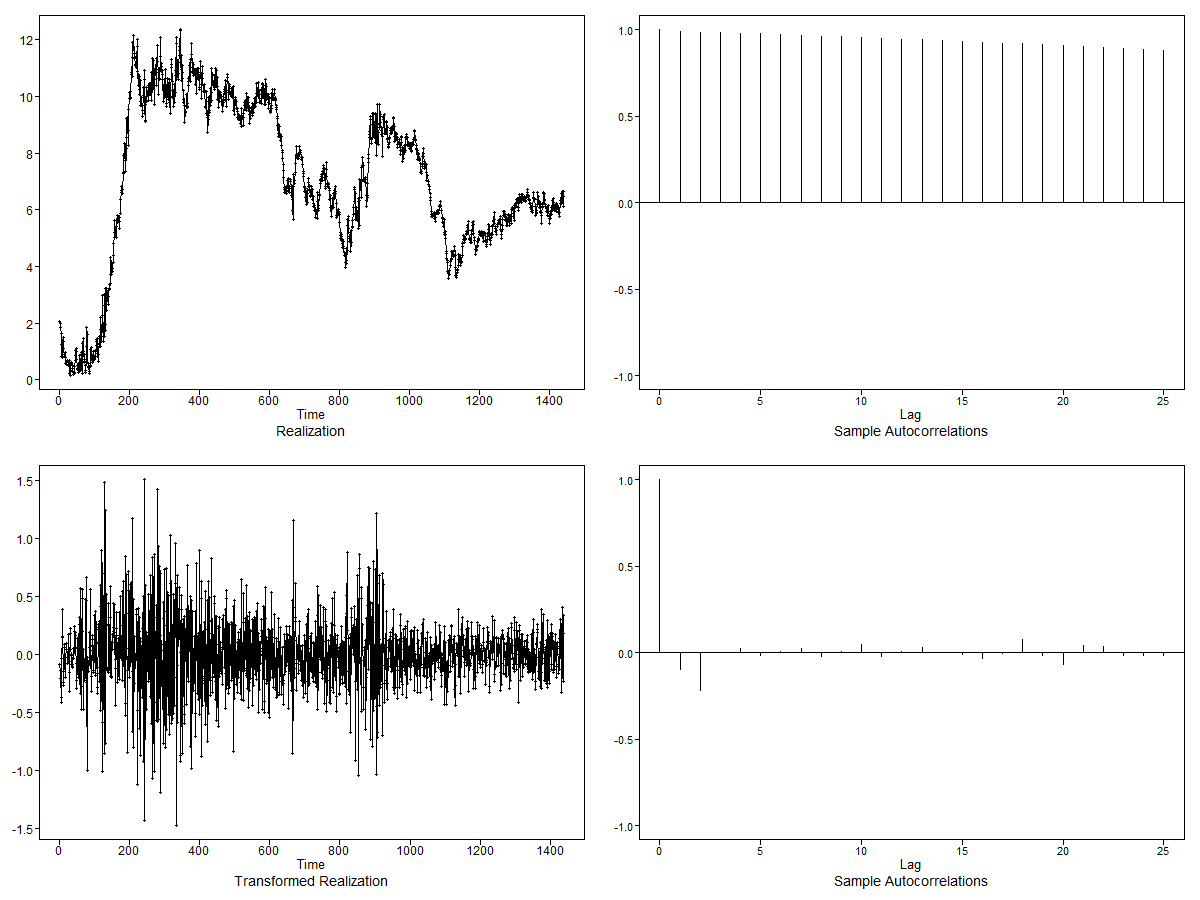
\includegraphics[width=0.75\textwidth]{apr_20_differenced.png}
  \caption{April 20, 2016 horizontal wind speed data before and after first order differencing.}
  \label{fig:apr20differenced}
\end{figure}

In examining the plots above, it appears that the differencing has successfully stationarized the data although there remains a change in variance at around time t = 1000 that we will have to address. The residuals are indicative of an MA(2) component remaining in the data, but given that MA processes are known to not be good representations of real-world processes, we searched for other AIC-based model fit recommendations and selected an ARMA(5,2) to fit on this differenced data.

\begin{figure}
  \centering
  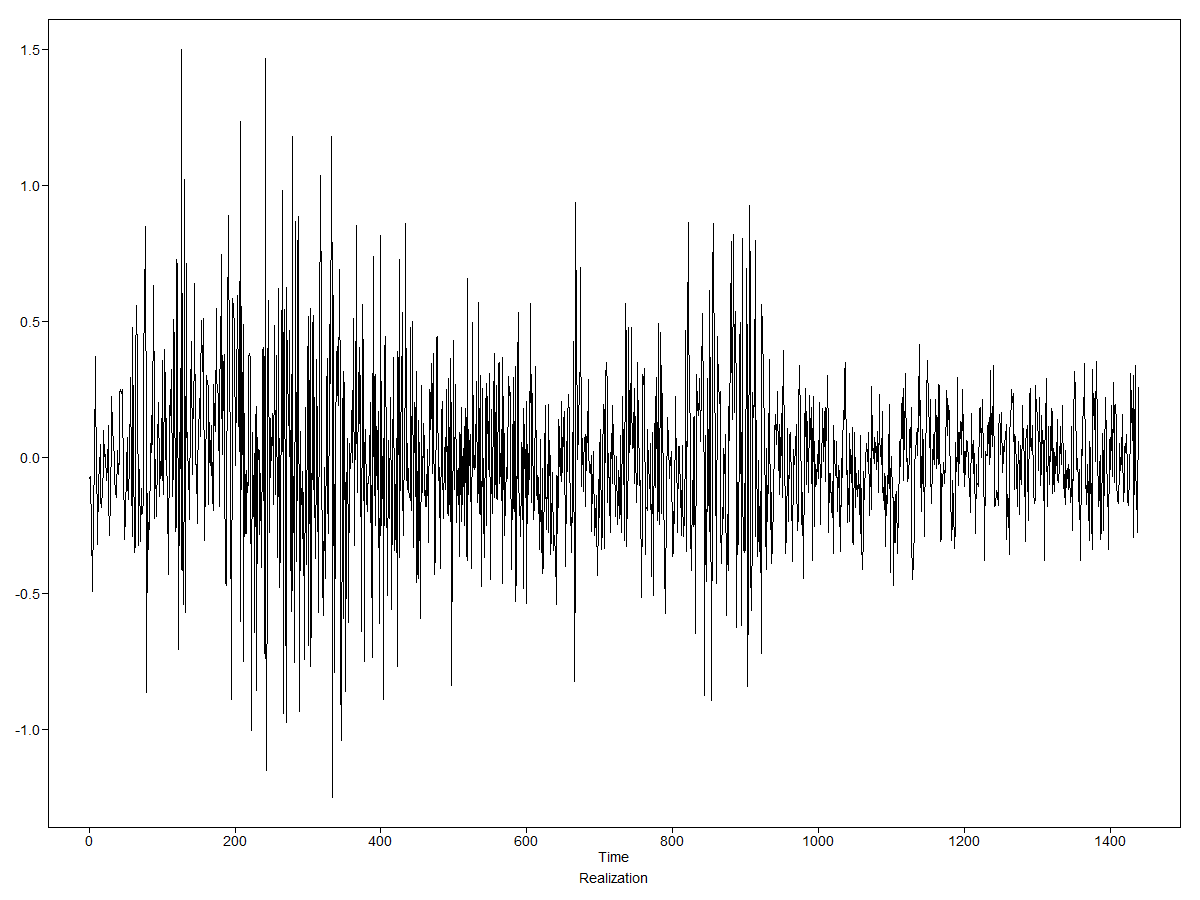
\includegraphics[width=0.75\textwidth]{apr_20_residuals.png}
  \caption{Residuals of the 20 April, 2017 data after applying an ARIMA(5,1,2) model.}
  \label{fig:apr20residuals}
\end{figure}

The above residuals visually appear to constitute white noise that is confirmed by examination of the ACF plot and through conducting statistical tests to confirm white noise. A Ljung-Box test performed on the residuals at at K =24 and K = 48 (p-values of .94 and .22 respectively) both fail to reject the null hypothesis that the residuals constitute white noise.

\begin{figure}
  \centering
  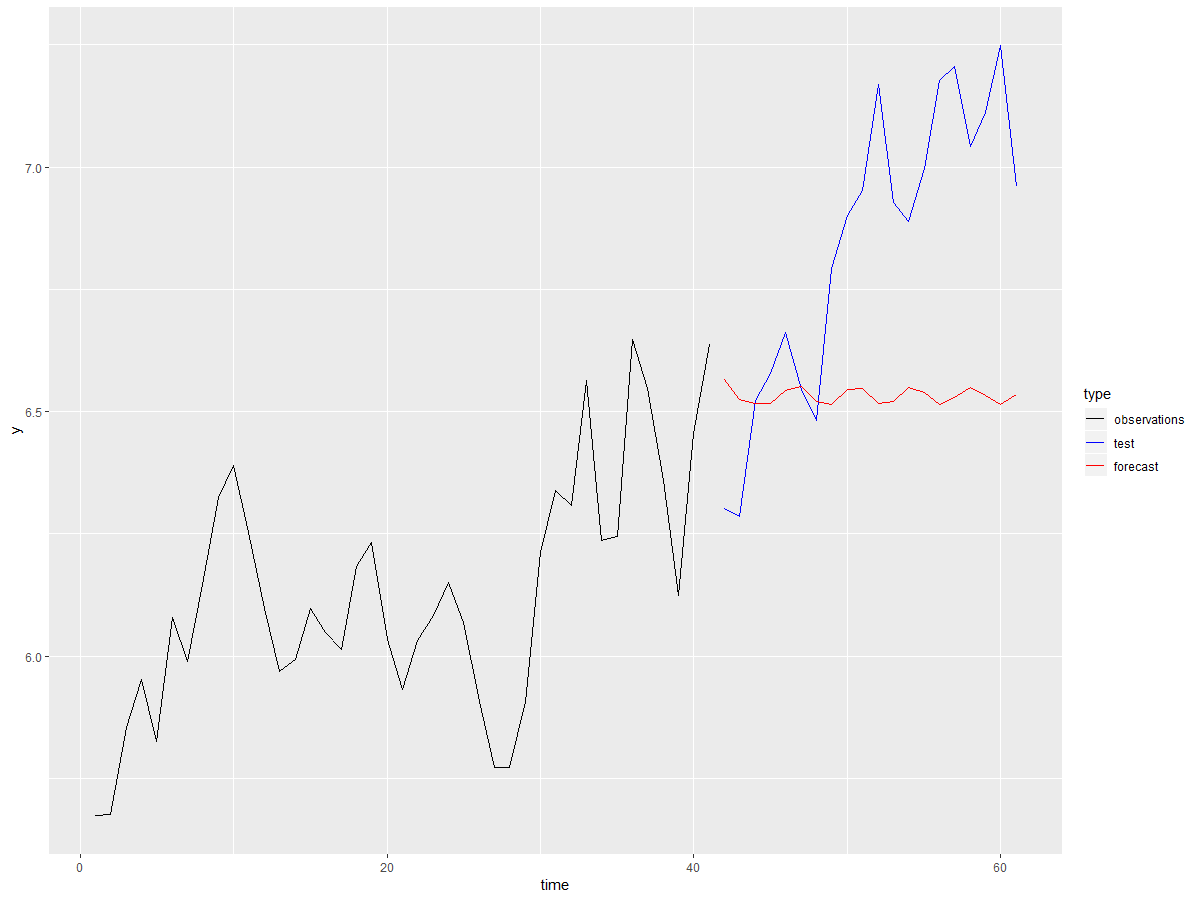
\includegraphics[width=0.75\textwidth]{apr_20_arima_forecasts.png}
  \caption{Forecasts for 15 minutes ahead using fitted ARIMA(5,1,2) model on 20 April data.}
  \label{fig:apr20arimaforecast}
\end{figure}

As the $t_0$ + 15 minute forecast using the ARIMA model in the figure above shows, the differenced term in the model dominates the behavior and forecasts are largely centered around the last observed value with some small cyclical behavior. When comparing these forecasts against the last 15 observed values, the forecasts achieve an Average Squared Error (ASE) of 0.18.

\subsection{Vector Autoregressive Model (VAR)}

In an attempt to improve this initial model, we next attempted to fit a Vector Autoregressive Model (VAR model) to the data with additional exogenous variables consisting of horizontal wind direction, average temperature, average air pressure and average humidity. A VAR selection procedure identified a K of 12 that provided optimal fit values by AIC.

\begin{figure}
  \centering
  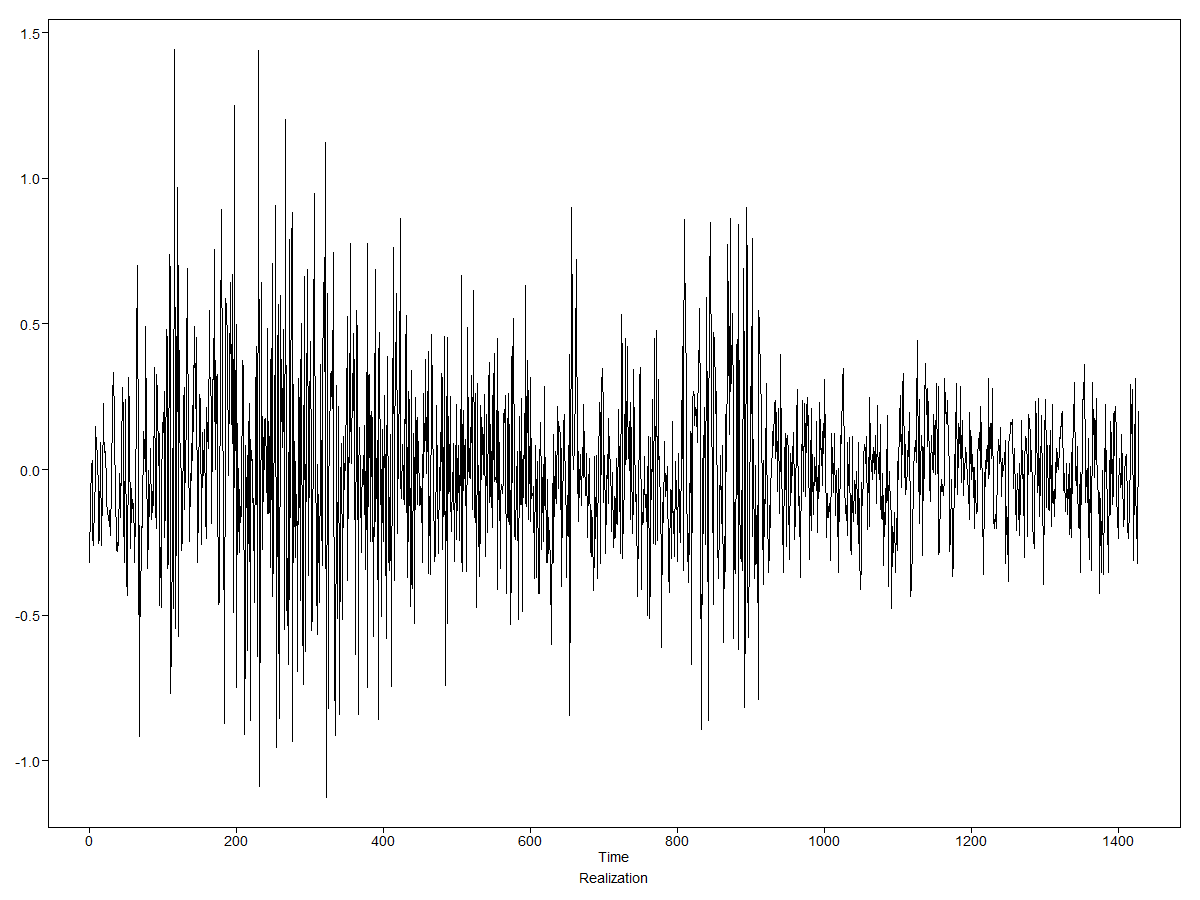
\includegraphics[width=0.75\textwidth]{apr_20_var_residuals.png}
  \caption{Residuals after fitting the 20 April data with a VAR model and K = 12.}
  \label{fig:apr20varresiduals}
\end{figure}

Looking at the residuals of this data we can see that the residuals are again observably white. Ljung-Box confirms this at K = 24 and K = 48 (p-values of .91 and .28 respectively).

\begin{figure}[H]
  \centering
  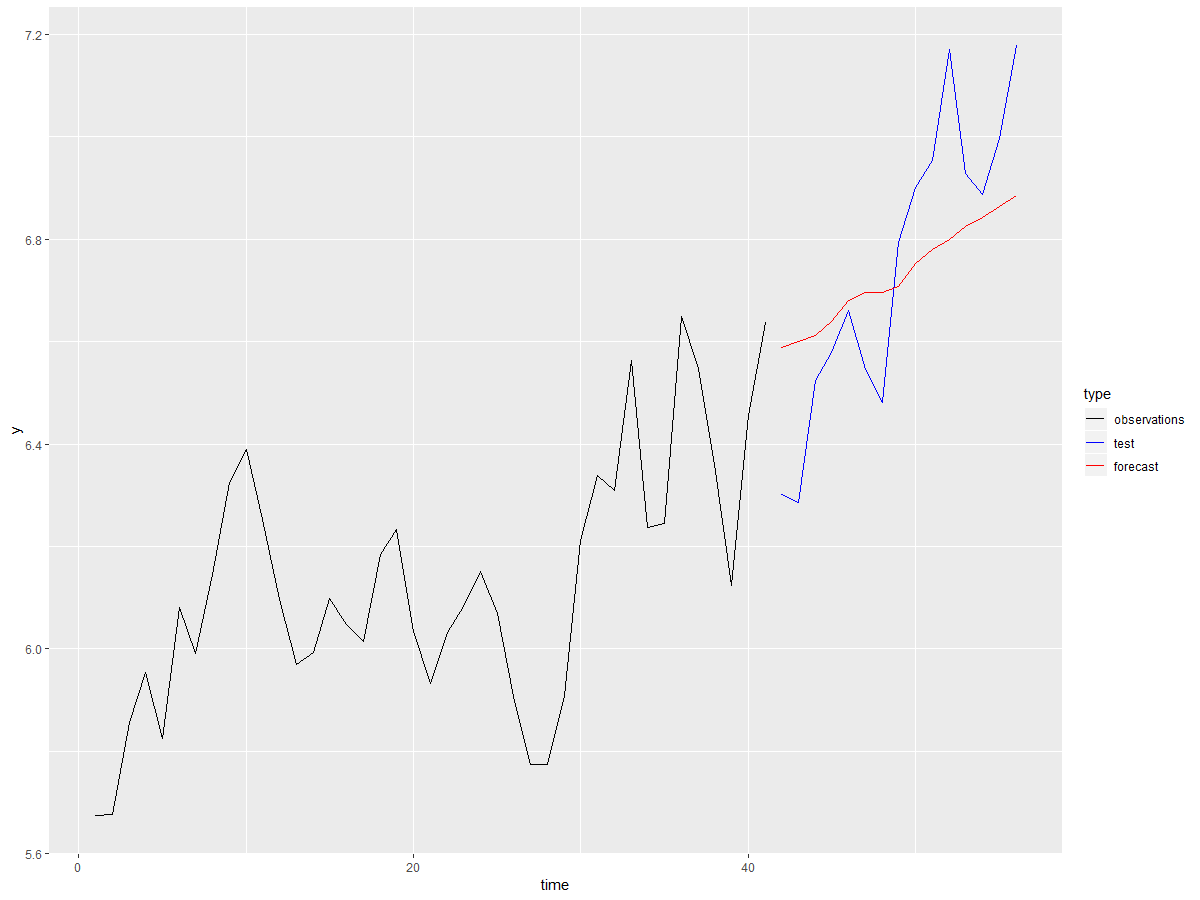
\includegraphics[width=0.75\textwidth]{apr_20_var_forecasts.png}
  \caption{Forecasts using the 20 April data with a VAR model and K = 12.}
  \label{fig:apr20varforecasts}
\end{figure}

Forecasts using the VAR model as displayed above appear to provide a more satisfying fit to the forecasts of the wind value, a fact that is reinforced by the improved ASE of 0.038.

\section{Ethical Considerations}

\subsection{Data Use and Protections}

The Department of Energy is a cabinet-level agency that has missions in both energy and national security related matters. Its purpose is to implement polices that support national energy security and promote technological innovation in nuclear power, fossil fuels, and alternative energy sources. While much of the offshore wind energy lidar buoy data is associated with the Department of Energy, the data is buoy wind speed testing data that is openly available to the public and not considered a national security risk. Pacific Northwest National Labs, a Federally Funded Research and Development Center (FFRDC), cannot place any further restrictions on the data that were collected using public funds.

Department of Energy provides the buoy LIDAR data consistent with the guidelines associated with Open Data defined in the open data handbook. \cite{opendatahandbook} This stipulates that data is available to all and for free use, as long as the original source of the data has been cited.

All data used was further reviewed by the research team to ensure protection of national security interests and avoid personal privacy information violations.

\subsection{Potential Conflicts of Interest}

No member of the research team has an identified conflict of interest associated with the data or the outcomes of the research. One member of the research team is a U.S. Government employee, but is not involved in energy policy, energy data analysis, or any matter related to the subject of this research. Another member of the research team is an employee of a national energy firm, but works in evaluating property tax compliance and cost evaluation and is similarly not involved in the wind energy or portfolio investment aspects of the company's operations.

\subsection{Ethics of Wind Energy}

It is beyond the scope of this project to evaluate in detail all the ethical risks of the promotion of wind energy. Generally, wind projects can interrupt flight paths and migratory patterns of some types of birds and bats leading to the deaths of many animals. Additionally, some individuals living near wind farms have surveyed negative feedback towards the aesthetics and noise caused by the turbines. With the adverse risks to wind energy, it is important to consider the placement of wind turbines in areas where the negative effects are minimized. Offshore wind turbines may limit these impacts, but pose other challenges to the communities and environment near where they are deployed.

Some community action to oppose offshore wind turbines as a blight on offshore views and due to other perceived environmental impacts have been documented. (citation needed) Wind turbines over the water can be moved to locations an acceptable distance to lower noise and visual obstructions for humans. Offshore wind turbines can also be placed in locations with lower impacts to nature. Wind energy is considered a viable alternative to fossil fuels which is generally accepted to cause more harmful impacts to nature and global climate change. Fossil fuels when consumed in large quantities to generate power for cities and significant populations can cause air pollution harmful to the health of people. Wind energy does not negatively impact air quality and therefore is an acceptable energy producing alternative.

\section{Advisors}

In order to gain assistance in guiding this research, the team has reached out to a number of both Southern Methodist University faculty members and academic / professional researchers in the field of wind energy. To date we have secured the following interest:

\begin{itemize}
  \item Dr. Y. Ding, Texas A\&M University: Although Dr. Ding is likely unable to act as our formal advisor, he has expressed willingness to respond to our specific questions related to the methodologies outlined in his book and to help steer our analysis when needed.
  \item Dr. B. Sadler, Southern Methodist University: Dr. Sadler has expressed willingness to help guide the time series aspects of our analysis, but is unable to act as our advisor due to other commitments.
  \item Dr. A. Gorton, Pacific Northwest National Labs: Dr. Gorton is one of the lead researchers of the DOE BUOY LIDAR project. She is considering specific research questions that may be of interest to the effort and ways in which we might contribute.
  \item Mr. B. Blanchard, Southern Methodist University: We have sought out Mr. Blanchard for his expertise in applied machine learning technologies and are awaiting a response.
\end{itemize}

 \bibliographystyle{splncs04}
 \bibliography{proposal}

% End the document
\end{document}
